% !TEX root=/home/tavant/these/manuscript/src/manuscript.tex

\section{PIC simulation results of the Axial-azimuthal simulations}
  \label{sec-Zthetaresults}
  In this sections, we present the results of the \ac{2D} \ac{PIC} simulations using the test-case of Boeuf \citep{boeuf2018}, described in \cref{subsec-boeuf_description}\string; the parameters used for the simulations are given in \vref{tab-parameters-boeuf}.
  In this test-case, the ionization is fixed, consequently the breathing mode is absent.
  Thus, the simulation converges quickly toward a steady state.
  
  We use the test-case of Boeuf in three different cases\string:
  the first is the usual case, without the effects of the radial direction.
  It is expected to return the same results as obtained in \citet{boeuf2018}.
  The two other cases model the influence of the radial direction.
  Two values of the radial length are used\string: $L_R=4\,\centi\meter$ and $2\,\centi\meter$.

  
  \subsection{Simulation results\string: an overview} \label{subsec-boeuf-overview}
    As the ionization is not self-consistently modeled, the simulations converges after less than $10\,\micro\second$.
    \Cref{fig-overview_boeuf_neEx} shows the axial and azimuthal distribution of the azimuthal electric field $E_{\theta}$ and the electron density $n_e$ at $t=10\,\micro\second$ is the case where no radial losses are modeled.
    We see in both $E_{\theta}$ and $n_e$ the \ac{ECDI}, which wavelength is approximately $\lambda_{\theta} = 0.08\,\centi\meter$.
    The results observed are similar to the one presented by \citet{boeuf2018}, but in order to validate the results, an exhaustive comparisons has been conducted between seven independently developed \ac{PIC} codes on this specific case.
    A good agreements has been shown \citep{charoy2019}.

    \begin{figure}[hbt]
      \centering
      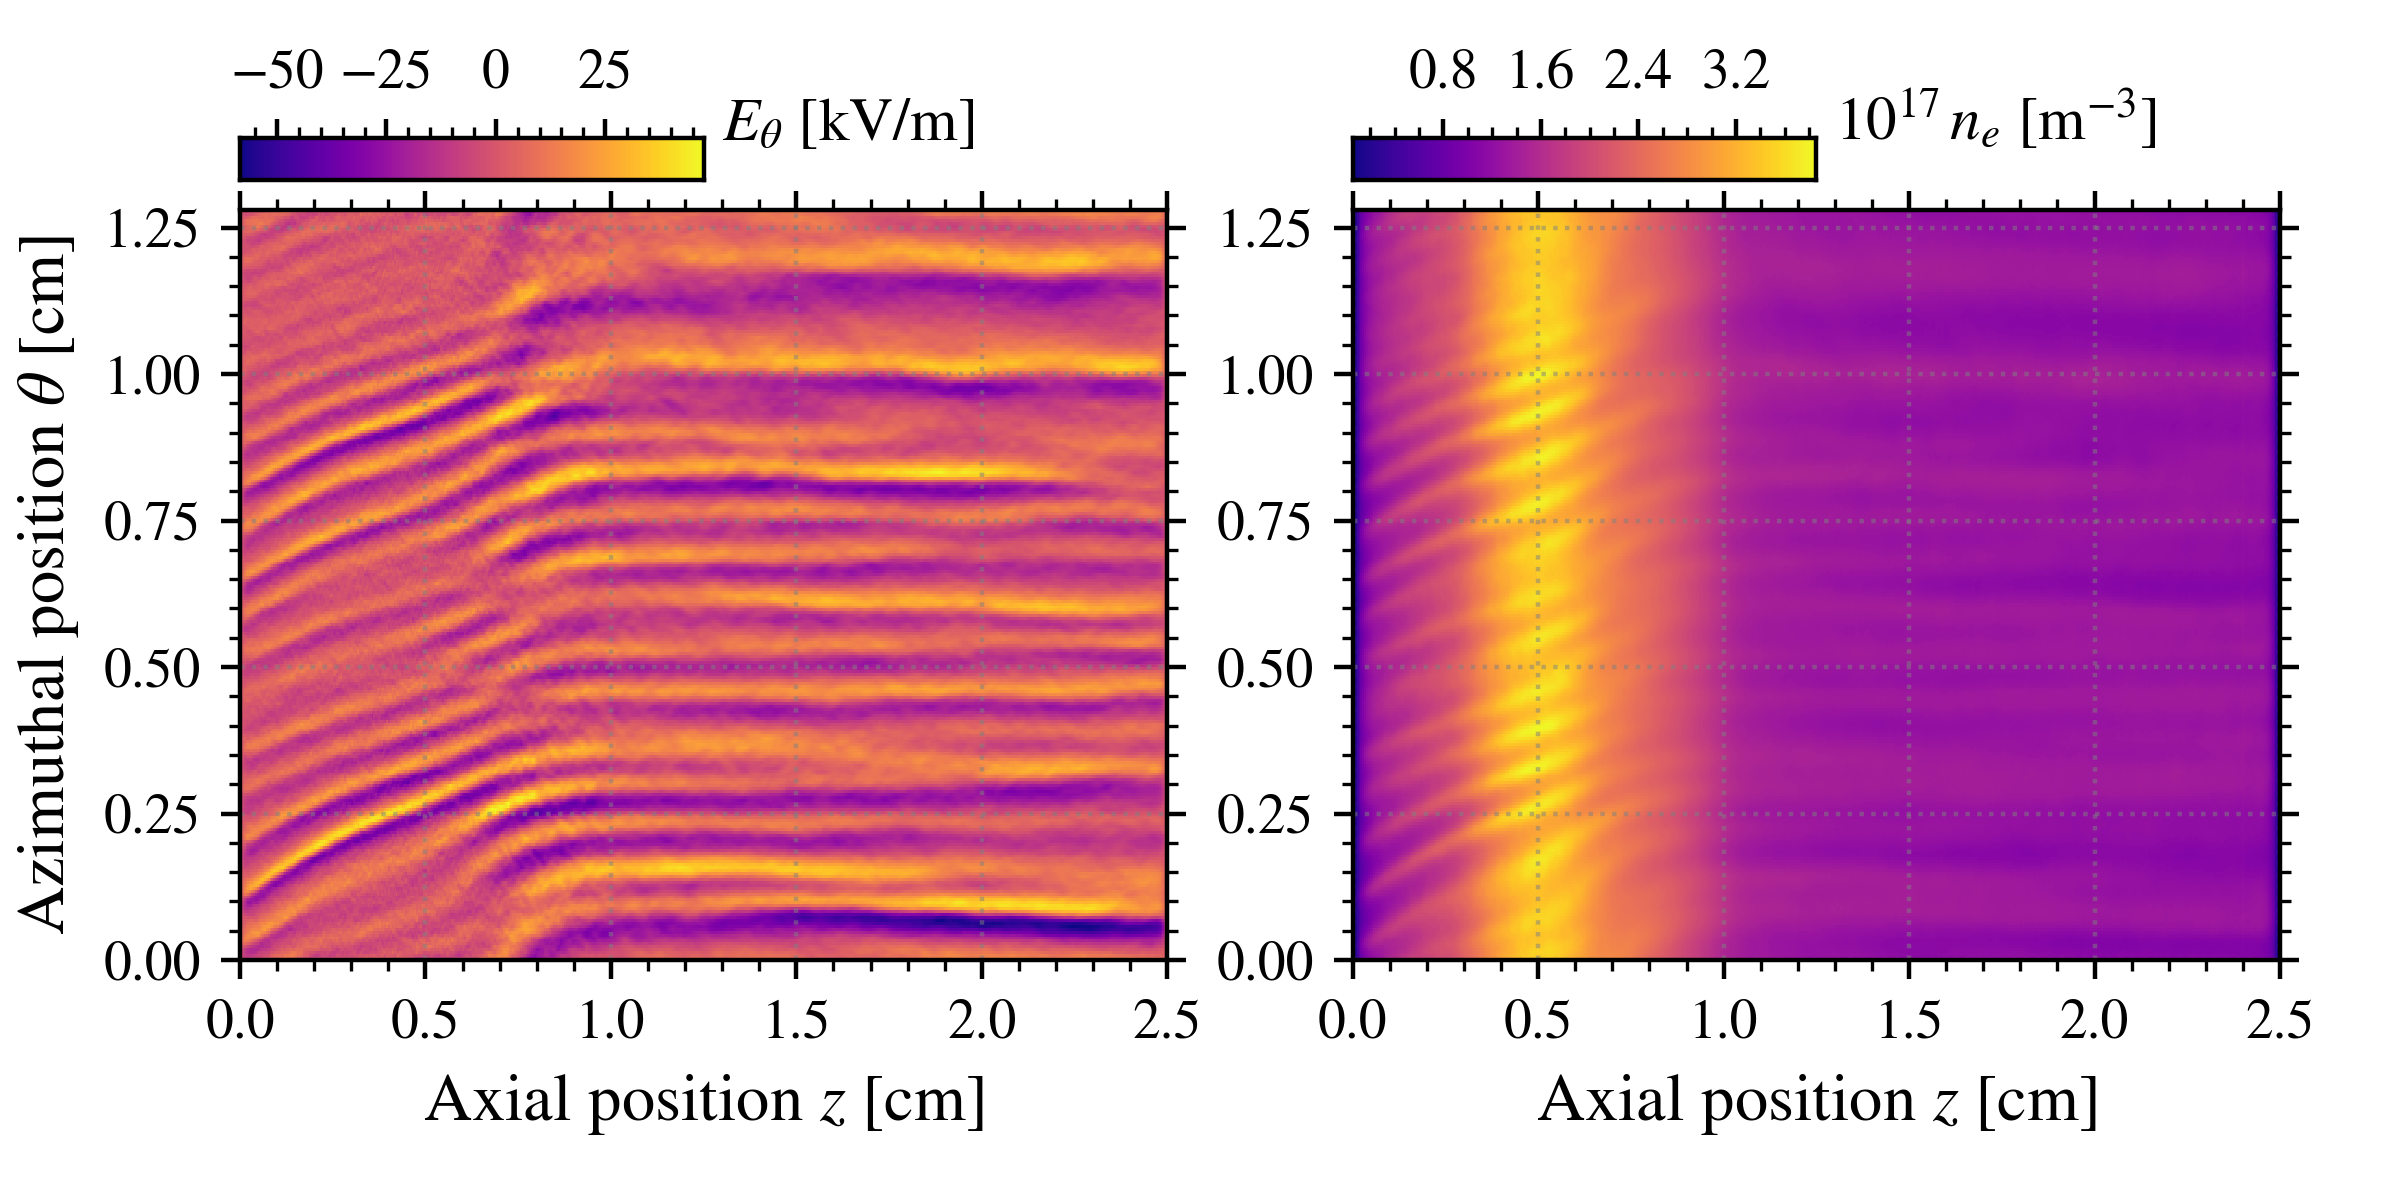
\includegraphics[width=0.9\textwidth]{Boeuf_example_t=8}
      \caption{ Axial-azimuthal distributions of (left) the azimuthal electric field $E_{\theta}$ and (right) the electron density $n_e$ at $t=10\,\micro\second$ for the test-case of Boeuf. } 
      \label{fig-overview_boeuf_neEx}
    \end{figure}

  \subsection{Simulation results\string: temporal evolution} \label{subsec-temp_boeuf}
    
    \Cref{fig-boeuf-temporal} presents the temporal evolution of the mean plasma density and temperature.
    We see that when the radial direction is modeled the density, the mean electron temperature, and the radial electron temperature are reduced, as expected when increasing the losses when the ionization source term is constant.

    \begin{figure}[hbt]
      \centering
      \begin{tabular}{cc}
        \subfigure{Boeuf_ne_temporal}{a}{20,20} &
        \subfigure{Boeuf_Te_temporal}{b}{20,20} \\
      \end{tabular}
      \caption{Temporal evolution of ({\bf a})  the mean plasma density, and  ({\bf b}) the  mean electron temperatures in the axial-azimuthal simulations, obtained with three different radial models. }
      \label{fig-boeuf-temporal}
    \end{figure}

    We see on \cref{fig-boeuf-temporal}.{\bf b} that the radial temperature remains constant when the radial direction is not modeled.
    This is due to the fact that the collisions are not modeled in the simulations, so that there is not momentum and energy transfer possible from the axial and azimuthal directions, and the radial direction.
    However, we know from the radial-azimuthal simulations that there is a transfer of energy between the axial direction and the radial direction, resulting in a plasma less anisotropic than observed here.
    This aspect is discussed latter in \cref{subsec-MCC_boeuf,subsec-radial-heating}.
    With the radial losses, the radial temperature decreases from the initial temperature $\Te=5\,\volt$ to $\Te_R\simeq 2.2$ and $ 3.3\,\volt$ for $L_R=2$ and $4\,\centi\meter$, respectively.
    The total temperature $\Te$ shows a similar decrease with the increase of the radial losses.

  \subsection{Simulation results\string: averaged axial profiles} \label{subsec-axial_boeuf}

    \Cref{fig-boeuf_axialone,fig-boeuf_axialtwo}  show the axial profile at steady-state of several plasma quantities.
    The variables are averaged in the azimuthal direction and in time during the steady-state between $t=8$ and $t=10\,\micro\second$.
    The results  obtained with three different radial models are overlaid.
    \cref{fig-boeuf_axialone}.{\bf a} shows the axial electric field $E_z$.
    The differences in $E_z$ are small, but we can still distinguish that the amplitude of $E_z$ is reduced with the increased radial losses.
    The electron density $n_e$ shown in \cref{fig-boeuf_axialone}.{\bf b} is almost not affected, except in for $z>1\,\centi\meter$, where the electron losses at the wall can be seen.

    \begin{figure}[hbt]
      \centering
      \begin{tabular}{cc}
        \subfigure{Boeuf_electric_field}{a}{30,22} &
        \subfigure{Boeuf_ne_axial}{b}{30,24} \\
      \end{tabular}
      \caption{Averaged axial profiles at steady state of ({\bf a}) the axial electric field $E_z$, ({\bf b}) the mean plasma density obtained with three different radial models for the simulation case of Boeuf. }
      \label{fig-boeuf_axialone}
    \end{figure}

    \Cref{fig-boeuf_axialtwo} shows the axial profiles of the electron axial density current and the electron temperatures.
    In contrast to $n_e$ and $E_z$, the electron temperatures are reduced by the radial losses in each direction ($\Te{}_{,\theta}, \Te{}_{,R}, \Te{}_{,Z}$).
    The radial temperature $\Te{}_{,R}$ is reduced uniformly everywhere, but the two other temperature are mostly affected before the axial position of their maxima, at approximately $z=0.8\,\centi\meter$.
    Surprisingly, as a first approximation, the radial losses should not reduce the axial and azimuthal temperatures.
    Indeed, if we suppose that the distribution function has separated variables
    \[ f(\vect{v_e}) = f_r(v_{e,r})f_{\theta}(v_{e,\theta})f_z(v_{e,z}), \]
    then the absorption of electrons with high radial energy does not modify the distribution function in the other directions.
    
    The electron heating comes principally from the Joule heating $\vect{J_e} \cdot \vect{E}$.
    As axial electric field $E_z$, seen in \cref{fig-boeuf_axialone}.{\bf a}, is almost unaffected, the difference in the electron temperature necessarily comes from the differences in the axial electron current.
    The axial electron density current $J_{e, z}$ is shown in \cref{fig-boeuf_axialtwo}.{\bf b}.
    It is more significantly reduced by the radial losses.
    
    \begin{figure}[!hbt]
      \centering
      \begin{tabular}{cc}
        \subfigure{Boeuf_Te_axial}{a}{25,80} &
        \subfigure{Boeuf_Je_axial}{b}{30,22} \\
      \end{tabular}
      \caption{Averaged axial profile at steady state of ({\bf a}) the  electron temperature, and ({\bf b}) the axial electron current density $J_{e, z}$, obtained with three different radial models for the simulation case of Boeuf. }
      \label{fig-boeuf_axialtwo}
    \end{figure}
    
    We observe a factor of two on $J_{e, z}$ between the case $L_R=2\,\centi\meter$ and the case without losses.
    As we have seen in \cref{fig-boeuf_axialone}.{\bf b} that the electron density is almost unaffected, this means that the electron axial velocity is reduced by the radial losses.
    \Cref{fig-mobility} shows the norm of the average electron velocity\[ v_{e,z} = | \frac{J_e}{e n_e }  | \]

    \begin{figure}[!hbt]
      \centering
      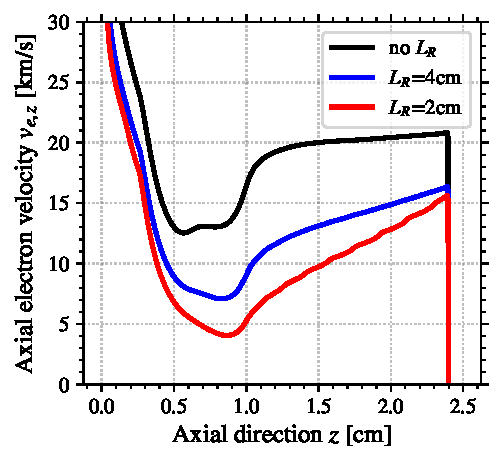
\includegraphics[width=\defaultwidth]{Boeuf_vez_axial.pdf}
      \caption{Axial profile of the norm of the axial electron velocity measured in the \acs{PIC} simulations for the three cases of radial losses.}
      \label{fig-mobility}
    \end{figure}

    We can see that the electron mobility is significantly affected by the radial losses.
    However, since the simulation is collisionless, the electron crossfield transport in the axial direction is only due to the azimuthal instability.
    It is confirmed by \Cref{fig-boeuf-instability}, that shows on the left the average standard deviation of the azimuthal electric field, and on the right the correlation term $R_{ei}$.
    We recall from \cref{sec-transport} that 
    \begin{equation} \label{eq-rei}
      R_{ei} =  - e < \dne \dEt >_{\theta},
    \end{equation}
    with $\dne$, and $\dEt$ the fluctuations of the electron density and azimuthal electric field, respectively.
    Moreover, we have from \cref{eq-mobeffsimple}
    \begin{equation*}
      \mu_e = \frac{< \dne \dEt >_{\theta} }{n_0 E_z}   \frac{1}{B_r}
    \end{equation*}


    \begin{figure}[!hbt]
      \centering
      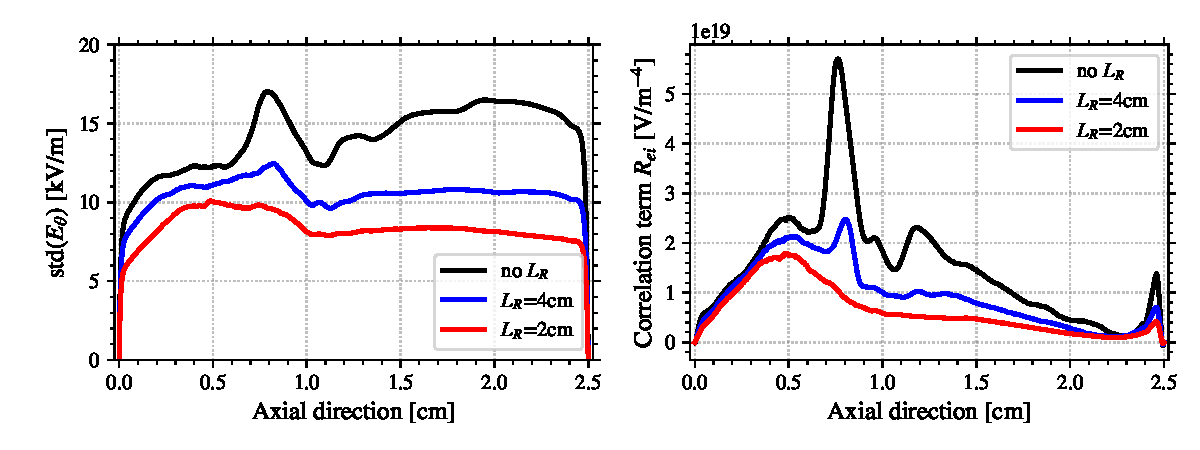
\includegraphics[width=\textwidth]{Boeuf_instability_characteristics}
      \caption{Axial profiles of the characteristics of the instability, (left) average of the standard deviation of the azimuthal electric field, (right) electron-ion friction force calculated by the correlation between $n_e$ and $\Te$.    }
      \label{fig-boeuf-instability}
    \end{figure}

    
    We observe in \cref{fig-boeuf-instability} that the amplitude of the instabilities, as well as the correlation term, are significantly affected by the electron radial losses.
    This explain the reduction of the axial electron current, but also the reduction on the Joule heating, which reduces the electron axial and azimuthal temperatures.

    \vspace{1em}
    To summarized the results presented in this section, we used a simple algorithm to model the radial particle losses in the \ac{2D} axial-azimuthal \ac{PIC} simulation.
    We observe almost no impact on the axial electric field $E_z$, and a slight diminution of the mean electron density $n_e$ (up to 20\% in total, but mostly present in the near-plume region).
    
    The electron temperature is also reduced, not only in the radial direction, where the radial losses have a direct impact, but also on the azimuthal and axial temperatures.
    This is consistent with the large reduction of the axial electron mobility, which lower the Joule heating.
    The reduction of the crossfield electron transport comes from the diminished amplitude of the azimuthal instability.
    In the next section, we analyze in more details the instability i order to explain the impact of the radial losses on the amplitude of the instability.
    In \cref{sec-rheating}, we will discuss radial heating of the electrons.


\afterpage{\clearpage}
